\documentclass{article}
\usepackage[
top    = 2.75cm,
bottom = 2.50cm,
left   = 3.00cm,
right  = 2.50cm]{geometry}
\usepackage{hyperref}
\usepackage{cite}
\usepackage{setspace}
\usepackage{algorithm}
\usepackage{graphicx}
\graphicspath{ {./images/} }
\title{\vspace{-2.0cm} A Generalizable Framework for Automated Cloud Configuration Selection \\ \vspace{0.5cm} \large Supervisors: Adam Barker \& Yuhui Lin}
\date{2019-06-06}
\author{Jack Briggs - 140011358 \\ MSc Data-Intensive Analysis}
\doublespacing
\begin{document}
\maketitle
\newpage
\section*{Abstract}
Outline of the project using at most 250 words
\newpage
\section*{Declaration}
I declare that the material submitted for assessment
is my own work except where credit is explicitly
given to others by citation or acknowledgement. This
work was performed during the current academic year
except where otherwise stated.
The main text of this project report is NN,NNN* words
long, including project specification and plan.
In submitting this project report to the University of St
Andrews, I give permission for it to be made
available for use in accordance with the regulations of the University Library. I also give permission for the title and abstract to be published and for copies of the report to be made and supplied at cost to any bona fide library or research worker, and to be made available on the World Wide Web. I retain the copyright in this work.
\newpage
\tableofcontents
\listoffigures
\newpage
\section{Introduction}
\textbf{Describe the problem you set out to solve and the extent
of your success in solving it. You should include the aims
and objectives of the project in order of importance and
try to outline key aspects of your project for the reader to look for in the rest of your report.}
\subsection{Background}
Cloud computing, specifically Infrastructure-as-a-Service (IaaS), has opened the doors to allow organizations and developers to utilize a diverse range of computer resources on demand without any up-front commitment or cost \cite{Armbrust2009}. These resources are generally provided in the form of Virtual Machines (VMs) with a diverse range of options, and correctly selecting the most appropriate cloud configuration for a given task or service can reduce costs for the user and free up underutilized resources for the cloud provider. Depending on the task, choosing a sub-optimal configuration can lead to up to 12 times higher costs in the worst case, but choosing randomly can lead, on average, to around twice the cost. \cite{Alipourfard2017}. While newer 'serverless' cloud options remove the challenge of selecting the optimal  configuration from the user, they instead  present providers the challenge of selecting optimal cloud configurations for a wide range of unknown applications.

\paragraph{}
Selecting the 'optimal' cloud configuration for a given job is not trivial, however. This is due to the large diversity in service, the difficulty in predicting performance, and the flexibility of the term 'optimal.' \\
The diversity in services provided by different cloud providers creates a large search space. At the time of writing, Amazon EC2\footnote{\url{https://aws.amazon.com/ec2/}} alone offers over 200 predefined instance models\footnote{\url{https://www.ec2instances.info}}, while Google Compute Engine\footnote{\url{https://cloud.google.com/compute/}} allows users to define their own machine types, ranging from small VMs with 1 vCPU and 1 GB of RAM to 96 vCPUs with 624 GB of RAM, and includes options for specifying the CPU platform or adding GPUs. \\
Once given a specific configuration, predicting its performance for a given job is difficult. A number of recent studies have shown that previously reported variability \cite{Leitner2014} in performance for different instances of a given instance type has dramatically improved \cite{Scheuner2018,Davatz2017,Laaber2019}, particularly for AWS, leading to much more consistent performance on a given instance type. However, even when stable, predicting performance is still far from trivial. \\ 'Larger' VM types may not provide improved performance \cite{Yadwadkar2017}, or may do so at a far less cost-efficient rate. Optimizing for a good mean performance may fail to optimize for the tail when variance or high stress leads to lower than expected performance. In addition, workload resource requirements are hard to model, with jobs using different resources at different times, and performance may have non-linear relationships with these resources\cite{Alipourfard2017}. A method to predict performance should account for these hurdles.
A costly option is to simply run the job or service itself on the instance type and measure the performance directly. For batch jobs, the cost of the initial performance testing can be offset by later repeats. In 2012, it was reported that up to 40\% of Microsoft's analytics jobs are recurring \cite{Agarwal2012,Ferguson2012b}. Another, faster, option is to run benchmarks or micro-benchmarks on the target machine, and use these to estimate performance. Benchmarking suites such as Cloud workbench \cite{Scheuner2018a} and CloudSuite \cite{Palit2016} allow application-specific performance prediction, and micro-benchmarking has shown success in rapidly estimating performance of appropriate applications with errors between 10-20\% \cite{Scheuner2018, Varghese2016a, Varghese2016}. However, using benchmarks to predict performance requires knowing how the benchmarked resources will relate to job performance, which limits the flexibility of an automated solution. \\
Finally, what is meant by the 'optimal' configuration may differ. For a batch job, it may simply be the cheapest option to complete the job, or it may be the cheapest option that can complete the job within a given time-constraint. For a service, there will likely be a trade-off between consistency, latency, and cost, and where the optimal balance lies will depend on the user's preferences or requirements.
In order to discover the optimal cloud configuration for a job, a user must first decide what 'optimal' means, find a way to evaluate the performance of a configuration given that metric, and either search or model the diverse range of available configurations according to this evaluation until they are confident they have found the best available configuration.

\subsection{Aims and Objectives}
We aim to design a framework and associated tool for searching through cloud configurations for any given cloud-based application, and estimating the optimal available cloud configuration according to a user-provided objective measure.
\paragraph{Objectives:}
\begin{itemize}
\item To provide a framework for optimizing the cloud configuration for any form of cloud-based application, such as a webserver or machine-learning job
\item Develop a tool that can provision instances, specified by various attributes, from multiple possible cloud providers
\item Develop a tool that deploys a given application on these provisioned instances and returns their logs for evaluation
\item Implement an optimization algorithm on top of the above tools.
\end{itemize}
\subsection{Contributions}
We successfully met all aims and objectives laid out in the above section. A framework was developed and is available at the project's Github\footnote{https://github.com/briggsby/AutomatedBayesCloudSelection}. We developed and evaluated tools, showing that we could effectively replicate and expand on previous cloud searching tools such as Cherrypick\cite{Alipourfard2017}.
We additionally showed how the optimization algorithm Bayesian Optimization was affected by different search configurations. It was shown that searching across multiple providers did not reduce the effectiveness of using Bayesian optimization, despite the increased search space. It was also shown that while running two concurrent jobs reduced search time without increasing search cost or reducing effectiveness, increasing the number of concurrent jobs further led to both reduced effectiveness and higher search costs, and did so with diminishing reductive effects on search time.
It was also clear from our testing that Amazon EC2 machines consistently outperformed Google Compute Engine machines of the same instance category and vCPU number at video transcoding operations.

\section{Literature Survey}
\textbf{Surveying the context, the background literature and any
recent work with similar aims. The context survey
describes the work already done in this area, either as
described in textbooks, research papers, or in publicly
available software. You may also describe potentially
useful tools and technologies here but do not go into
project-specific decisions.}

% Existing work (Cherrypick (BO), PARIS, Ernest)
% Technical background (Terraform, Spearmint)

%First ways of actually evaluating the performance of a black box app
%Then describing previous configuration testers 
	% How Cherrypick was extremely effective and used an open-source BO tool spearmint that will be used
%Problem of making it work across multiple providers, leading to modern Infrastructure as code developments


\section{Requirements Specification}
Previous solutions to the problem of automated cloud configuration selection have focused on specific use-cases or application types, and have not provided any associated functional implementation.  Our design should be generalisable to any form of application deployed on the cloud, and should be able to recreate previous solutions. This paper should also come with an associated implementation, which can at least perform a Bayesian Optimization-based search for a given docker container containing a batch job or benchmark.

The solution should be capable of:
\begin{itemize}
\item Performing optimization algorithms wrapped around some deployment schema
\item Specifying cloud configurations based on a collection of input variables
\item Provisioning specified cloud configurations from multiple possible providers
\item Installing or setting up a container platform such as Docker onto provisioned instances
\item Deploying user-specified images onto provisioned instances
\item Retrieving logs from remotely deployed containers
\item Interpreting logs into single values which are returned to the optimization algorithms
\end{itemize}

The solution will, preferably, also be capable of running multiple concurrent sample 'jobs' for the optimization algorithms.
While many of these requirements are either met, or a means of performing them provided through APIs or other tools, we hope to provide an implementation that combines them into a single generalizable automated cloud selection tool. 


We should be capable of effectively replicating previous optimization methods such as CherryPick\cite{Alipourfard2017}, Ernest\cite{Venkataraman2016}, or PARIS\cite{Yadwadkar2017} in our system. We must also ensure that our solution is capable of provisioning instance and deploying applications on machines from multiple providers, and as such cannot rely on any provider-specific API or command-line interface, but will use one of several Infrastructure-as-code tools now available. This is just one of the ways that extending a search space to include multiple providers causes additional problems. To ensure that any optimization algorithm will be effective, we must encode the search space for cloud configurations such that instances are described in terms of a set of descriptive variables. At the time this is written, no universal or cross-provider API exists in the Infrastructure-as-code tool we implemented (Terraform) that allows instance types to be looked up based on their specifications, and so we must develop our own method for describing them for lookup by the optimization algorithms.  

\section{Design}
\begin{figure}[!ht]
  \centering
   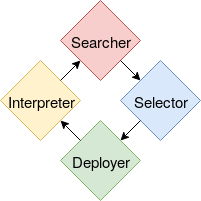
\includegraphics[scale=0.8]{Design}
  \caption{A diagram of the design.}
  \label{fig:design}
\end{figure}

In any optimisation process, the value of some objective function is minimised or maximised by adjusting its input variables or parameters. An optimisation algorithm begin with an initial guess of these variables and iterates through improved estimates until they terminate, hopefully providing an estimated solution. \cite{Nocedal2006} In our generalized case, the optimisation method and objective function are both unknown, but we know that our objective function will always involve selecting some cloud configuration based on the inputs that describe that configuration, deploying some application onto this configuration, and interpreting its performance to give some objective measure.

This process can be broken down into four components: A Searcher, which runs the optimisation algorithm, testing out various inputs in an attempt to maximise or minimise the objective function; a Selector, which interprets the inputs to determine what cloud configuration is being tested; a Deployer, which provisions the machines needed for that cloud configuration, deploys the application, and once it has terminated returns any required logs from it; and an Interpreter, which takes these logs to calculate the objective measure which is returned to the Searcher as the returned value for the objective function. A diagram of this breakdown is shown in figure \ref{fig:design}.

It is assumed that in the vast majority of cases, the user would provide their own Interpreter and Selector. Interpreters and Selectors are very dependent on the form these logs will take, and the form the search space will take, and are extremely hard to generalise. For this reason, the modular design of our solution should make it simple for any component to be supplied or replaced by the user. In only some cases should the user need to provide their own Deployer. Applications can often be contained within Docker containers, and aside from occasional setup, for example in multi-node clusters or multi-container applications, a Deployer which provisions a given configuration from a given provider, and then deploys and attaches to a user-provided docker image to collect its logs will be sufficient.  Only in rare cases would the user be required to provide their own Searcher. This is because optimization algorithms can be applied to any deployment, with only small modifications necessary in rare cases for specific cases, and an implementation of Bayesian Optimization will be provided.

\subsection{Searcher}
The Searcher component performs an optimisation algorithm, such as Bayesian optimization, coordinate descent, random search, or exhaustive search, and drives the optimization process by iterating through potential input variables. For each set of these inputs, it take a sample from a single 'job,' where it runs through a single loop of the other three components. The constraints for these input variables must be specified, by describing their type (integer, float, categorical) and limits. A description of how to model cloud configurations into a set of variables is done in the Selector section. Ideally, we want our searcher to be capable of performing multiple jobs concurrently.

Here we describe and compare the design considerations of two important examples of searchers which will be used for the evaluation of our implementation.

\subsubsection{Exhaustive search}
In an exhaustive search, every possible combination of the inputs is sampled, giving a complete analysis of the entire search space. This obviously takes many samples, $n * \prod_{i=1}^{j} x_{i}$ where $x_{i}$ is the number of options for the \textit{i}th of J variables, and n is the number of samples taken from each configuration. This results in a large or even infinite search cost and time, but is almost certain to return the optimal result, depending on the amount of randomness involved in sampling.

\subsubsection{Bayesian Optimization}
Bayesian Optimization is an optimization method specifically designed for situations where the objective functions itself is unknown beforehand and expensive to perform, but can have its outputs directly observed through experiments\cite{Snoek2012}. It models the objective function as a stochastic process, a 'prior function,' and computes its confidence intervals based on samples. Using these confidence intervals and a pre-defined acquisition function it decides future samples to take based on where there it estimates there to be the most potential gain. By this process Bayesian Optimization can find optimal or near-optimal solutions for any non-parametric problem in a relatively small number of samples compared to other optimization methods. In addition, whereas other methods, such as exhaustive search, may handle uncertainty through sampling results from the same inputs multiple times, Bayesian Optimization can incorporate this uncertainty into its estimates, further reducing the number of samples needed.

There are a number of possible prior functions, acquisition functions, and stopping conditions that can be used with BO, and the Cherrypick paper goes into detail on the reasoning behind which options are best for cloud configuration selection specifically\cite{Alipourfard2017}. Some notable differences in our case, however, is that CherryPick was specifically focused on batch jobs, where what is measured is simply a function of an instance type's cost and its time taken to perform a given job. Its acquisition function is specified to this purpose, minimizing costs but biased towards configurations which satisfy a soft performance constraint by successfully performing the batch job within a given time. In our case, our acquisition function must be more general, and we will therefore be relying on the user to ensure that whatever objective measure it returned by their Interpreter has already taken into account soft or hard performance constraints such as this.

\subsection{Selector}
The Selector interprets the variables provided by the Searcher component into the form of an available cloud configuration. Cloud configurations have a number of variables that can describe them, such as vCPU number, memory amount, disk speed, number of instances, instance category, machine type, and cloud provider. The selector must use whatever combination of these is provided and find either the exact or most similar cloud configuration available, passing this information on to the Deployer. In the tools used for our implementation, no cross-provider API was available to directly translate machine specifications into the virtual machine types available from different providers. 
% Though Apache libcloud does offer this


For finding an exact match, the Selector can simply lookup the appropriate instance type from a dataset according to the input variables stored as each instance type's attributes. Looking for a closest match rather than an exact one gives more flexibility in how the input variables can be encoded, but means more complicated decisions such as attribute priority must be made, and extra assurances made to not repeat unnecessary samples when multiple sets of inputs describe the same closest input type.

Whether using exact or closest match, it must be decided how to encode cloud configurations into a set of input variables. This problem is further complicated by the fact that constraints for certain inputs may depend on the values of others, as is often the case in cloud computing. Large memory amounts are often only available on machines with more vCPUs, and some providers may offer available configurations others do not. Google Cloud Platform allows users to specify custom machine types, but even these do not allow any possible combination (for example, Memory constraints are tied to vCPU number, and vCPU number must be divisible by 2).

Despite these problems, clear patterns prevail throughout leading cloud providers, such as separating machine types into categories equivalent to 'Compute-optimised', 'Memory-optimised', and 'Storage-optimized,' each with a set of machines with between 2 and 96 CPUs. In lieu of a cross-provider service to match a given specification to a specific cloud instance type, something which would be outside the scope of this project, these industry-standard categorisations can be used to encode the search space in a reasonable manner. Table \ref{tab:config-encode} shows an example of how we have used these patterns to encode 6 instance types into a set of 3 easily interpreted variables; Provider, vCPU number, memory, and machine category. A searcher tool could easily filter a dataset of this form to find the instance-type for a set of input variables.

\begin{table}[!t]
\centering
\begin{tabular}{ |c||c|c|c|c|  }
 \hline
 Instance Type & Provider & Category & vCPU Number & Memory \\
 \hline
 n1-standard-2    & GCE  & General & 2 & 7.50 \\
 n1-standard-4    & GCE  & General & 4 & 15.00 \\
 n1-standard-8    & GCE  & General & 8 & 30.00 \\
 c5.large         & EC2  & CPU & 2 & 4.00 \\
 c5.xlarge    & EC2  & CPU & 4 & 8.00 \\
 c5.2xlarge    & EC2  & CPU & 8 & 16.00 \\
 \hline
\end{tabular}
\caption{A possible way of separating instance types into 4 descriptive variables. Providers were either the Google Compute Engine (GCE) or the Amazon Elastic Compute Cloud (EC2)}
\label{tab:config-encode}
\end{table}


In the end,  however, the important features and constraints for the search space will differ for each user, and it may be beneficial to run multiple experiments in different search spaces before settling on a final decision for an instance type. While we provide in our associated implementation an example of how to encode and select available cloud configurations for our Bayesian Optimization tool, we think it best to ultimately leave it to the user to design and implement a Selector system that works well for their specific use-case.


\subsection{Deployer}
The Deployer deploys the user-provided application, batch job, or benchmark onto the selected cloud configuration, and collect any necessary analysis from it. Typically this will involve provisioning the necessary machines from the given provider, followed by deploying the given application onto these machines, and either collecting logs from them or from a networked instance or cluster. 

\subsubsection{VM Provision}
Aside from in serverless computing, the first step of deploying any cloud-based application is likely to be provisioning the virtual machines themselves from a cloud provider. The Deployer should be capable of requesting any virtual machine chosen by the Selector, regardless of provider. This can be simplified using Infrastructure as code (IaC) tools such as Terraform, which offers the ability to codify the APIs from many different providers into declarative configuration files. As long as configuration files and credentials for use by an IaC tool are supplied for each possible provider, then a Deployer can call the corresponding IaC tool to provision the machines. 
There are several requirements for the IaC tool that is used. As instance type and number of machines will be supplied by the Selector, and therefore cannot be known until the machines are provisioned, either they must be declarable as variables when the tool is run, or the configuration files must be suitable for automated editing just beforehand. Along with this, the tool must support multiple concurrent tasks with their own specifications and outputs, if we hope to allow the Searcher to take multiple samples at once.

\subsubsection{Docker Deployment}
Once the virtual machines themselves have been provisioned, the application must be deployed onto them. We have assumed that the application being tested is available in the form of a Docker image, and that the machines provisioned operate as either a Kubernetes based cluster or a single instance. While other forms of application or cluster architecture may be used, ready-made Kubernetes clusters are available on several major cloud providers. The modular design allows users to implement their own Deployers to deal with alternative situations. 

Both Kubernetes and Docker offer remote APIs. For Kubernetes clusters available on cloud providers, no set up is required, while for single machines the VM provisioner must install Docker and direct it to a public-facing port. The remote APIs can be utilized as long as the VM Provisioner is capable of returning the public facing IP of the provisioned machines, and that security credentials are provided. The Deployer must attach to any deployment, or wait for its completion, and obtain and return any and all logs it produces for use by the Interpreter.

\subsubsection{Simulated Deployment}
It may be advantageous, especially during debugging or if using a 'closest match' approach to configuration selection, to instead either simulate the response from provisioning and deployment of an application, or to return a previously sampled response. To this end, it may be useful to ensure full logs of any deployment are stored so that, if desired, future calls to 'Deploy' an already sampled configuration for a given application can simply be responded with a randomly distributed value based on previous results from the same configuration.

\subsection{Interpreter}
The Interpreter must interpret whatever logs and other information is returned by the Deployer, along with the cost of the cloud configuration provided by the Selector, in order to return an objective measure for the sampled cloud configuration. It is this returned value that the Searcher will be attempting to minimise or maximize. We leave it to the user to develop an Interpreter for their use-case. This will likely involve extracting relevant information from the deployed application's logs, and applying constraints based on the time taken or machine pricing. 

\section{Implementation}
Our solution was implemented with a combination of Bash scripts and Python 3. For Selector, Deployer, and Interpreter, a single core Python script was made to call user-specified functions from the three components. This script would be called by a Searcher component for each sampling job, taking the input variables as its parameters, and returning the objective measurement given from that configuration, as defined by the Interpreter. User-provided options, such as what Selector, Deployer, and Interpreter to use, as well as other user supplied variables can be provided in the form of a JSON file that is read and loaded as a Python dictionary by this core script. This dictionary is passed as input to each component, which are able to update it with any information needed by other components in the form of key-value pairs. At the end of any job, this dictionary object is saved in JSON format for later analysis and recovery of previous results.

\subsection{Searcher}
Exhaustive search was performed using simple shell commands. Bayesian optimization was performed using Spearmint, an implementation of BO written in Python. However, the latest available implementation of Spearmint was found to be outdated and incompatible with the latest versions of various Python modules used in later steps. 
Because of this, for the sake of generalisability we first updated Spearmint to be compatible with Python 3 and newer versions of its dependencies such as Google Protocol Buffers. This implementation of spearmint has been made available.\footnote{https://github.com/briggsby/spearmint3}

\subsection{Selector}
A CSV file was created with the following variables for the instance types used in our evaluation:

\begin{itemize}
\item API Name - Name of instance type used in that provider's APIs (string)
\item Provider - Cloud provider offering the instance type (string)
\item CPU - Number of vCPUs (float)
\item Memory - Amount of memory in GB (float)
\item Category - Category of machine type, such as Compute or Memory optimized, in a consistent form between providers (string) 	
\item Price - Hourly cost of the machine for an On-demand Linux image (float)
\end{itemize}

The selector loads this dataset as a Pandas dataframe, and filters it according to the input variables provided, and returns the API name and hourly cost for the cheapest option remaining.

\subsection{Deployer}
\subsubsection{VM Provisioner}
The first stage of any tested deployment was to first provision the necessary virtual machines from their cloud provider. To this end, a separate folder for each provider was created with a corresponding Terraform configuration file. The configuration files would, when applied using Terraform, provision a number of machines of a given type, and set up a publicly accessible Docker host on each machine. The number of machines, type of machines, and other important variables such as credentials file locations can be specified when the configuration plan is applied, or placed in a single 'tfvars' file in the same folder as our driving Python script. The Terraform plan outputs a timestamp, configuration details, and the public IP, which are used used by later Deployment steps.

It was important that we could run multiple Terraform plans at once, but using a separate configuration setup for every job would lead to extremely large disk usage and overhead from downloading necessary modules into every folder. Because of this, each deployment uses a different 'local back-end,' storing the state files in a separate folder. Output values are only taken from the standard output returned when the configuration plan is first applied, as attempting to get the outputs later can lead to returning outputs from different back-ends when separate deployments attempt to obtain this information at the same time.

We used a Python library python-terraform\footnote{https://github.com/beelit94/python-terraform} for our implementation. The public IP address is used with the Python Docker library to deploy docker images onto the provisioned instances.

\subsubsection{Ping server}
In some cases, a separate server may be used to simulate network requests to a tested application. In these cases, a separate Kubernetes cluster was provisioned beforehand, and its details and credential file locations written into the configuration file. This allows the pinging Docker image to, after the application is deployed successfully on the tested instances, be deployed on the Kubernetes cluster and its logs returned.

\subsection{Interpreter}
For Interpreter functions used in our evaluation, simple Python scripts were implemented that used regular expressions to extract relevant information from the returned logs. These values, often scores from some benchmark, were then divided by the hourly price of the instance.
This is not likely to correspond to any real metric used by a business, as even small advantages over a competitor may lead to a dramatic uptake in users, but was thought to be an effective enough measure to use for evaluating our implementation.

\section{Evaluation}
To demonstrate the effectiveness of the implementation of our framework, we wanted to show that it could replicate the methods set out in the Cherrypick paper \cite{Alipourfard2017} by performing Bayesian Optimization to attempt to find an optimal configuration for a given deployment. We then wanted to use the same implementation to perform multiple exhaustive searches so that the results from Bayesian Optimization could be properly compared to the real average results.

\paragraph{}
Video streaming is one of the most common services for which cloud servers are used, where video files are transcoded to an appropriate file type and streamed to an end-user's device\cite{JunXin2005, Lottarini2018}.
The deployment to be used was originally planned to be Cloudsuite3's media streaming benchmark\cite{Palit2016}, however this was found to be extremely variable and dependent entirely on network bandwidth, and so instead the vBench video transcoding benchmark was used\cite{Lottarini2018}. Our objective function measured an instance type's relative rate of transcoding of a single 5 second 1920x1080 video file, returning a score of 0 if the quality was below a given threshold, divided by the hourly price of that instance. Effectively, we maximised the rate of transcoding a unit of video length at a sufficient quality per hourly cost. We had hoped to show that incorporating the hard constraint on video quality within the value returned by the Interpreter, rather than within the Acquisition function as was done in Cherrypick, did not hinder the optimization process, however no instance type tested failed to achieve the threshold video quality in any case.

\paragraph{}
For choosing the boundaries of the search space, we decided to reduce costs by using only machines ranging from 2 vCPUs to 8 vCPUs. This was also convenient as to use more powerful machines would have required requesting additional raised quotas from the providers used, and so would be less easily replicable by others wishing to repeat our evaluation. As we wanted to show that the implementation worked with multiple providers, and were were ensuring our input variables matched exactly to an available instance type, we could not rely on Google cloud platform's custom machine types and had to find some way to categorize possible variables. Rather than including memory as a variable, CPU instead was coded as a categorical variable (2, 4, or 8), along with machine category (General, Memory, CPU), each with a different amount of memory. Table \ref{tab:instance-types} show which machine types corresponded to each option. 

\begin{table}[!hb]
\centering
\begin{tabular}{ |c||c|c|  }
 \hline
 & \multicolumn{2}{|c|}{Provider} \\
 \hline
 Machine Category & Amazon EC2 & Google Compute Engine \\
 \hline
 General& n1-standard & m5\\
 Memory & n1-highmem  & r5\\
 CPU    & n1-highcpu  & c5\\
 \hline
\end{tabular}
\caption{Machine types corresponding to different instance categories for the two providers}
\label{tab:instance-types}
\end{table}

For more resource-intensive situations, the search space could follow this same pattern, with the CPU variable extended, possibly instead as an integer between 1 and 6 which 2 is raised to the power of to determine vCPU number, as this covers many of the available CPU options.

The 18 machine types decided upon (3 vCPU numbers for 3 machine categories for the 2 providers) were stored in a single CSV dataset for use with the instance Selector. A vBench Deployer was used which utilized Terraform to provision a single instance of the given machine type, on which the remote docker API was used to deploy and collect logs from an docker image containing vBench. An Interpreter then isolated the vBench score from these logs, and divided it by the hourly cost of that machine type to return the final value.

Where not otherwise specified, statistical results are quoting the p-values returned from a Tukey's Honest Significant differences test to correct for multiple comparisons. Analysis was performed in RStudio\cite{R, RStudio}, and full logs as well and scripts used for analysis are available on the project's Github repository.

\paragraph{}
The results of the exhaustive search are shown in figures \ref{fig:vBench-scores} and \ref{fig:vBench-values}. The raw scores (time taken to transcode relative to the reference) show clear overlap between many possible configurations. While in general they show a significant difference between 2 vCPUs and either 4 ($P < .001$) or 8 ($P < .001$) vCPUs, where the score increases with vCPU number, they show less certain differences between 4 and 8 ($P = .066$), dependent on the provider and machine category, suggesting either diminishing returns or a limit of the benchmark to utilize all vCPU cores.
 
\begin{figure}
  \centering
   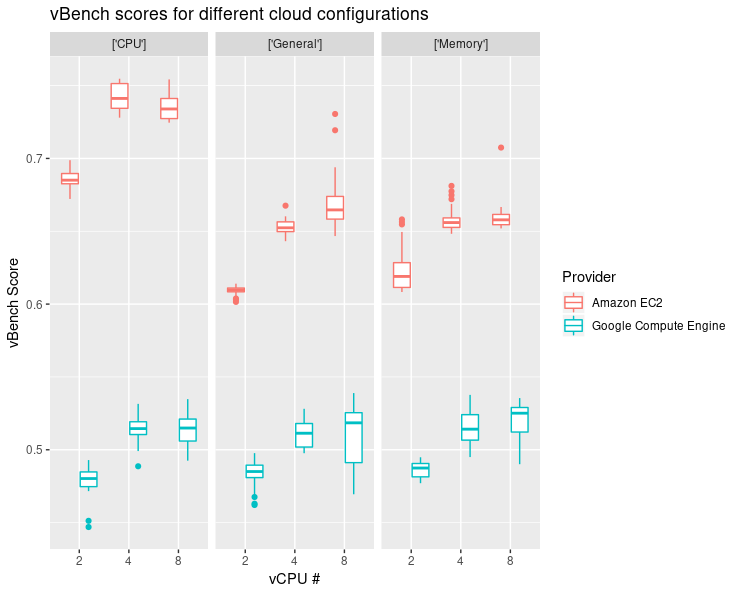
\includegraphics[scale=0.8]{vbench_scores}
   \caption{Distribution of vBench scores}
  \label{fig:vBench-scores}
\end{figure}
\begin{figure}
  \centering
   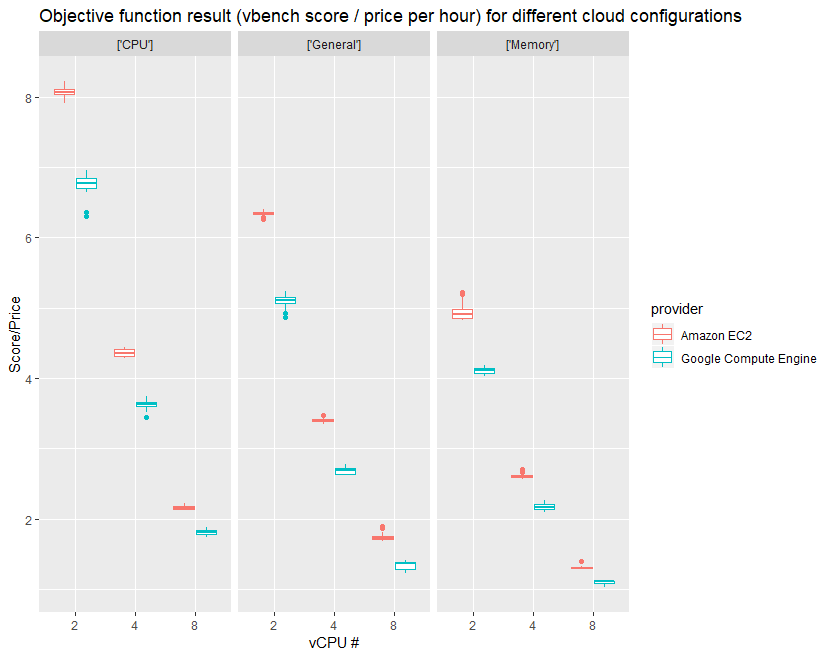
\includegraphics[scale=0.8]{vbench_values}
   \caption{Distribution of objective function values}
  \label{fig:vBench-values}
\end{figure}
\begin{figure}
  \centering
  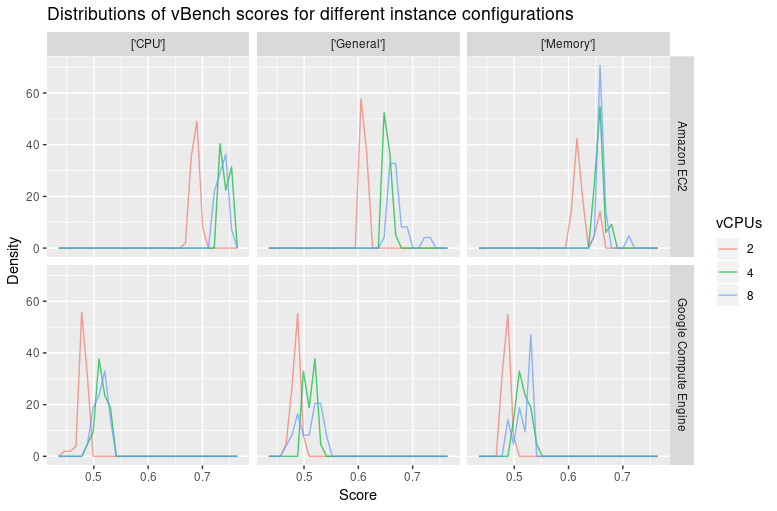
\includegraphics[scale=0.7]{vbench_dists}
  \caption{Distribution of vBench scores in frequency polygons}
  \label{fig:vBench-dists}
\end{figure}

However, once the scores are divided by that machine's hourly costs, there is much less overlap. A clear optimal configuration can be seen in the c5.large machine type, if one is purely interested in getting the most video transcoding for a given cost. The c5.large machine was significantly better than the next best option, the n1-highcpu-2 ($P < .001$). Amazon EC2's  machine types consistently outperformed Google Compute Engine's equivalents of the same category and vCPU number at both raw score (Anova, $F = 32111.456, P < .001$) and value for money (Anova, $F = 22710.7, P < .001$). However, despite this general trend, the provider seemed to be the least important factor in determining the optimal configuration. For example, the n1-highcpu-2 still gave significantly better values than the m5.large ($P < .001$), or the c5.xlarge ($P < .001$) making it the second most cost-efficient option. 

\begin{figure}
  \caption{Optimal configurations suggested after convergence for Bayesian Optimization searches}
  \label{fig:bo-results}
  \centering
  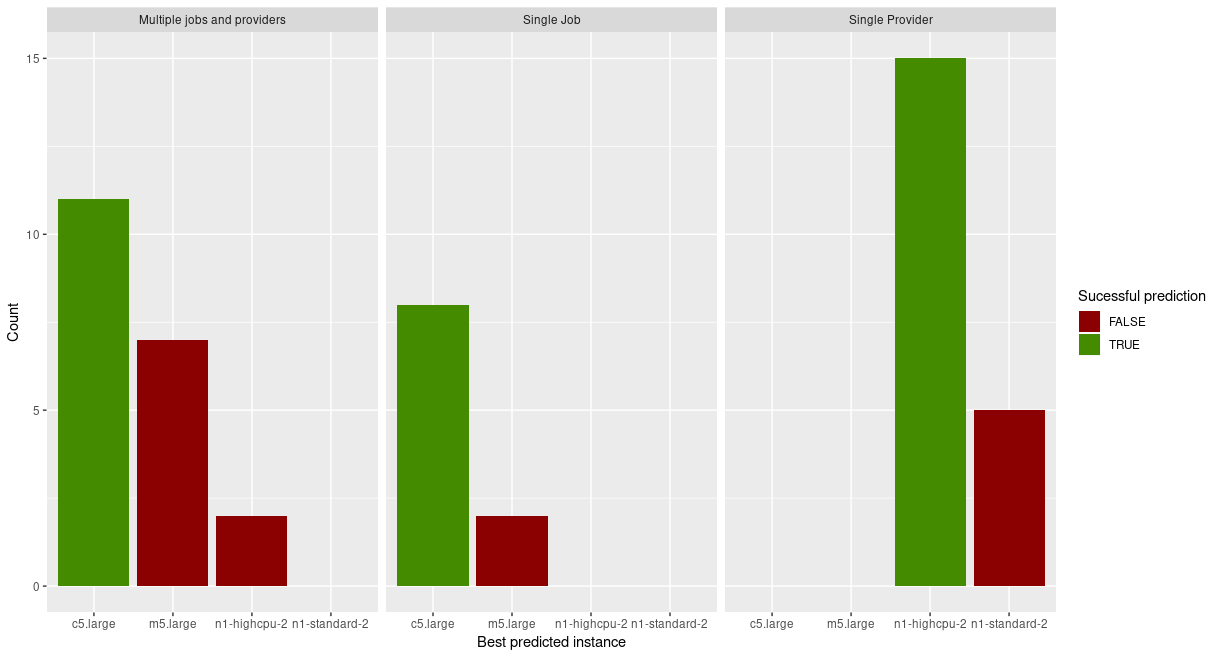
\includegraphics[scale=0.5]{bo_results}
\end{figure}
\begin{figure}
	\centering
	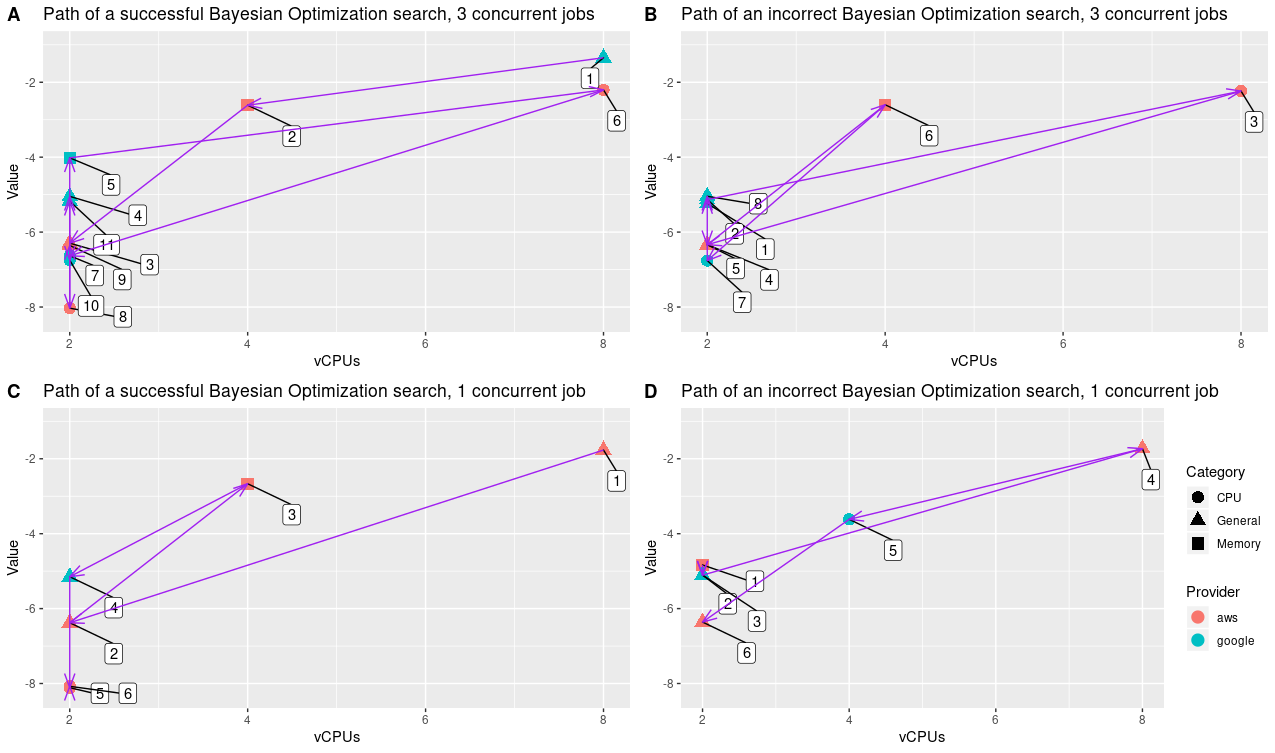
\includegraphics[scale=0.4]{paths}
	\caption{Paths of example Bayesian Optimization jobs}
	\label{fig:paths}
\end{figure}

\paragraph{}
With the exhaustive search complete, we then used a Spearmint based searcher to perform a Bayesian Optimization search, assuming low noise (-1 to 1) and using the same stopping conditions as used by default in the Cherrypick paper \cite{Alipourfard2017}, namely when the Expected improvement (EI) is less than 10\%, and at least 6 samples have been taken. We were able to successfully run this experiment with both multiple and single providers, as well as with between 1 and 3 multiple concurrent jobs. The results from these experiments are shown in figure \ref{fig:bo-results}, while examples of the job paths taken during them are shown in figure \ref{fig:paths}. Figure \ref{fig:bo-boxplots} shows the difference in values returned, time taken, and estimated search cost for different experiment configurations.


When testing instances from only a single provider, and running only a single concurrent job at any time, we were able to replicate the findings of the Cherrypick paper \cite{Alipourfard2017}. In 85\% of cases (17 of 20 experiments), Bayesian Optimization was able to reach the same conclusions as Exhaustive search in only 6-12 samples. 

Despite increasing the number of providers, with only a single concurrent job running, we were also able to replicate the previous results, with the correct optimal instance predicted in 18 out of 20 evaluations, in only 6-11 samples. For our evaluation, despite doubling the search space, Bayesian Optimization was no less effective.  It may be interesting to note, however, that the incorrectly predicted instance in both failed cases was not the second but third best choice, coming from the same provider rather than the other, resulting in a reduction in the mean score/cost value by ~21.3\%.  

By allowing 2 concurrent jobs to be run at any one time, the time taken for the search was reduced to less than half that of before ($P < .001$), without any significant loss in value returned ($P = .97$) or rise in search cost ($P = .79$). However, increasing the number of concurrent jobs higher, to 3, causes a dramatic reduction in effectiveness. The probability of returning a sub-optimal instance increases, while increasing the search cost compared to 2 concurrent jobs ($P = .024$) without any significant further decrease in search time ($P = .46$). To ensure this held true even in a reduced search space, the experiment was repeated with 3 concurrent jobs but only a single provider, to similar results.


\paragraph{}
Having performed evaluation on our implementation for a deployment of a simple docker container, effectively corresponding to running a single batch job or benchmark and interpreting the results, we then wanted to evaluate the same technique applied to an web-based application, which may be better evaluated through its responses to a client. For this a single 5-node Kubernetes cluster was set up for the same of sending repeated requests to the evaluated deployment, as described for the 'Pingserver' deployer and interpreter. This experiment is much more intensive to perform exhaustive search for, as it would require separate pinging clusters to be set up for every sample. The mean response time for requests of a normally distributed load was divided by the hourly cost of the instance to give maximised value. From the samples taken during 10 repetitions of this experiment, it seemed that there were no significant difference between the two optimal configurations of c5.large and m5.large ($\Delta \bar{x}=0.0001, P \approx 1.000$), which the predictions correctly converged upon in all cases.

\begin{figure}
  \caption{Values, search costs and times for different Bayesian Optimization searches. Single large outlier removed from search time graph from Single provider, 3 concurrent jobs.}
  \label{fig:bo-boxplots}
  \centering
  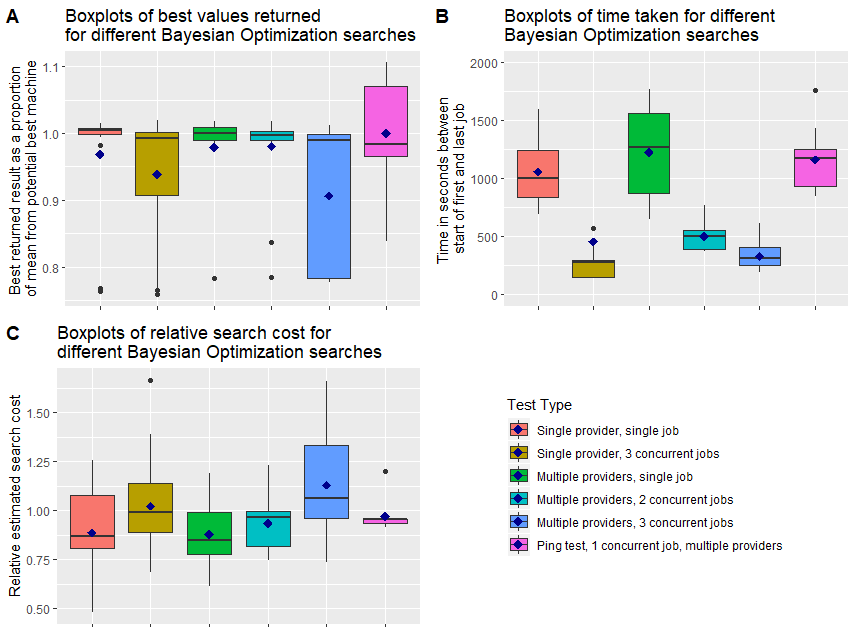
\includegraphics[scale=0.5]{bo_boxplots}
\end{figure}

\section{Critical discussion}
\textbf{You should evaluate your own work with respect to your
original objectives. You should also critically evaluate
your work with respect to related work done by others.
You should compare and contrast the project to similar
work in the public domain, for example as written about
in published papers, or as distributed in software available to you. }

As mentioned, the evaluation above likely does not correspond to comparisons with which to base real deployment decisions on. In reality, a small increase in transcoding speed may lead to a far greater increase in customer uptake, rather than the effectively 1:1 ratio between price and transcoding speed assumed in the experiment. However, the evaluation shows that the methodology works very well with a given objective score measure, and it would be trivial for a new objective function to be implemented with a different relationship between the score, price, and 'value' of a given configuration.
\subsection{Future extensions}
% There is a really good space to try this with serverless computing, but cloud run is currently not supported with terraform making this more difficult.
% If time allows could write a quick bash script to try this.
% When limited to google the search space becomes much better suited for Bayesian Optimization because of the non-categorical choices with vCPU and Memory amounts
% So it turns out Apache Libcloud exists, which is probably better than Terraform in absolutely every way for hte purposes of what we are doing. It even allows looking up available nodes from a provider according to specifications for vCPU number, disk size, disk type, etc., and provides automatic pricing information. It is also already natively written in Python. It is on the Apache 2.0 license.
\section{Conclusions}
\textbf{You should summarise your project, emphasising your
key achievements and significant drawbacks to your
work, and discuss future directions your work could be
taken in.}
\newpage
\bibliographystyle{ieeetr}
\bibliography{Dissertation}
\newpage
\section*{Appendices}
\subsection*{Testing Summary}
\subsection*{User Manual}
\end{document}